\section{Package Model}\begin{figure}[h!]
\begin{center}
	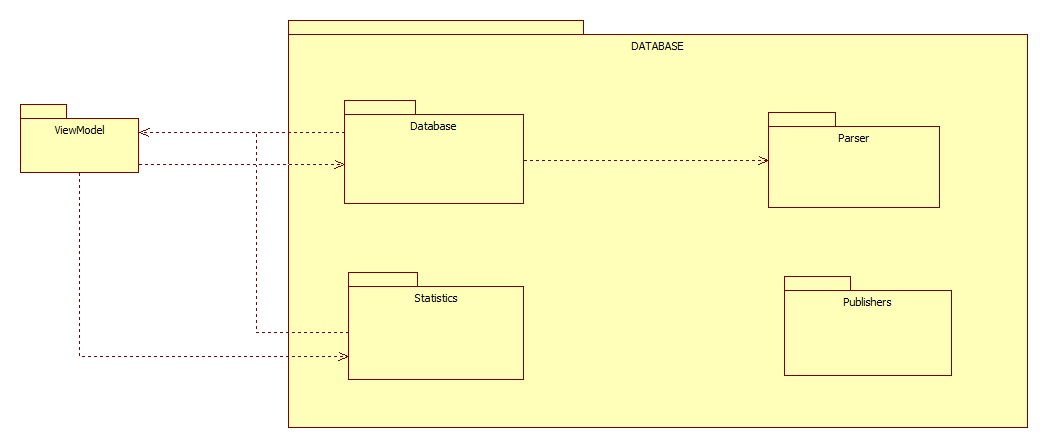
\includegraphics[scale=0.4]{../images/ModelPackage.jpg}
\end{center}
\end{figure}
\subsection{Model::Database}
\subsubsection{Model::Database::QuizManager}
\begin{figure}[h!]
\begin{center}
	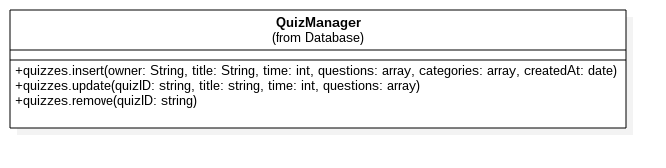
\includegraphics[scale=0.4]{../images/Model/Database/QuizManager.png}
\end{center}
\end{figure}
\begin{itemize}
\item\textbf{Funzione del componente:} la classe permettera' l'inserimento, la lettura e la rimozione di questionari all'interno della collezione
\item\textbf{Relazioni d'uso con altre componenti:}
Questo elemento è in relazione con:
\begin{itemize}
	\item Model::Publishers::QuizPublisher\\
	\item Model::Statistics::Statistics\\
\end{itemize}
\item\textbf{Metodi}:
\begin{itemize}
	\item\code{+ quizzes.insert()} : Metodo per aggiungere un nuovo quiz al database\\
	\textbf{Parametri}:
	\begin{itemize}
		\item\code{owner: string}\\
		\item\code{title: string}\\
		\item\code{time: int}\\
		\item\code{questions: array}\\
		\item\code{categories: array}\\
		\item\code{createdAt: date}\\
		\textbf{Precondizioni}: Vengono richiesti i dati necessari per la creazione e il salvataggio di un quiz\\
		\textbf{Postcondizioni}: Il quiz e' stato salvato correttamente nel database e crea una entry corrispondente nella collezione delle statistiche\\
	\end{itemize}
	\item\code{+ quizzes.update()} :  Metodo per modificare un quiz nel database\\
	\textbf{Parametri}:
	\begin{itemize}
		\item\code{quizID: string}\\
		\item\code{title: string}\\
		\item\code{time: int}\\
		\item\code{questions: array}\\
		\item\code{categories: array}\\
		\textbf{Precondizioni}: Vengono richiesti i dati necessari per la modifica di un quiz\\
		\textbf{Postcondizioni}: Il quiz e' stato modificato nel database\\
	\end{itemize}
	\item\code{+ quizzes.remove()} : Metodo per rimuovere un quiz dal database\\
	\textbf{Parametri}:
	\begin{itemize}
		\item\code{quizID: string}\\
		\textbf{Precondizioni}: Vengono richiesti i dati necessari per la rimozione di un quiz\\
		\textbf{Postcondizioni}: Il quiz e' stato rimosso dal database e le statistiche ad esso associate vengono anch'esse rimosse\\
	\end{itemize}
\end{itemize}
\end{itemize}
\newpage

\subsubsection{Model::Database::QuestionManager}
\begin{figure}[h!]
\begin{center}
	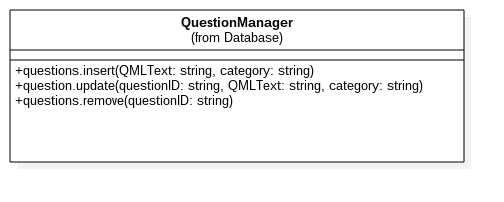
\includegraphics[scale=0.4]{../images/Model/Database/QuestionManager.png}
\end{center}
\end{figure}
\begin{itemize}
\item\textbf{Funzione del componente:} la classe permettera' l'inserimento, la modifica e la rimozione di singoli quesiti all'interno della collezione
\item\textbf{Relazioni d'uso con altre componenti:}
Questo elemento è in relazione con:
\begin{itemize}
	\item Model::Publishers::QuizPublisher\\
	\item Model::Statistics::Statistics\\
	\item ViewModel::Interpreter::Interpreter\\
\end{itemize}   
\item\textbf{Metodi}:
	\begin{itemize}
		\item\code{+ questions.insert()} : Metodo per aggiungere un nuovo quesito al database\\
		\textbf{Parametri}:
			\begin{itemize}
				\item\code{QMLtext: string}\\
				\item\code{category: string}\\
				\textbf{Precondizioni}: Vengono forniti i dati necessari per la creazione e il salvataggio di un nuovo quesito (il testo QML e la categoria vengono immessi dall'utente mentre data e utente corrente sono informazioni già presenti il sistema al momento della richiesta)\\
				\textbf{Postcondizioni}: Il quesito e' stato salvato correttamente nel database se viene rispettata la sintassi QML, altrimenti viene restituito un messaggio d'errore\\
			\end{itemize}
		\item\code{+ questions.update()} : Metodo per modificare un quesito nel database\\
		\textbf{Parametri}:
			\begin{itemize}
				\item\code{questionID: string}\\
				\item\code{QMLtext: string}\\
				\item\code{category: string}\\
				\textbf{Precondizioni}: Vengono forniti i dati necessari per la modifica di un intero quesito o di sue parti (es. solo alcune parti del testo o cambio di categoria)\\
				\textbf{Postcondizioni}: Il quesito e' stato modificato nel database se viene rispettata la sintassi QML, altrimenti viene restituito un messaggio d'errore\\
			\end{itemize}
		\item\code{+ questions.remove()} : Metodo per rimuovere un quesito dal database\\
		\textbf{Parametri}:
			\begin{itemize}
				\item\code{questionID: string}\\
				\textbf{Precondizioni}: L'utente richiede l'eliminazione di un quesito\\
				\textbf{Postcondizioni}: Il quesito e' stato rimosso dal database\\
			\end{itemize}
	\end{itemize}
\end{itemize}
\newpage

\subsubsection{Model::Database::Search}
\begin{figure}[h!]
\begin{center}
	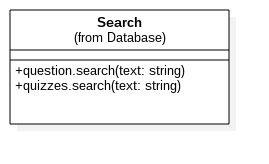
\includegraphics[scale=0.4]{../images/Model/Database/Search.png}
\end{center}
\end{figure}
\begin{itemize}
\item\textbf{Funzione del componente:} la classe permettera' la ricerca di sottostringhe in singoli quesiti o in diversi questionari 
\item\textbf{Relazioni d'uso con altre componenti:} 
Questo elemento è in relazione con:
\begin{itemize}
\item Model::Publishers::QuizPublisher\\
\item Model::Publishers::QuestionPublisher\\
\end{itemize}  
\item\textbf{Metodi}:
\begin{itemize}
	\item\code{+ question.search()} : Metodo per ricercare una stringa all'interno di tutte le domande\\
	\textbf{Parametri}:
	\begin{itemize}
		\item\code{string: string}\\
		\textbf{Precondizioni}: Viene fornito il parametro che si vuole ricercare\\
		\textbf{Postcondizioni}: Vengono restituite tutte le domande che contengono il parametro\\
	\end{itemize}
	\item\code{+ quizzes.search()} :  Metodo per ricercare una stringa all'interno di tutti i questionari\\
	\textbf{Parametri}:
	\begin{itemize}
		\item\code{string: string}\\
		\textbf{Precondizioni}: Viene fornito il parametro che si vuole ricercare\\
		\textbf{Postcondizioni}: Vengono restituite tutti i questionari che rispecchiano i criteri di ricerca\\
	\end{itemize}
\end{itemize}
\end{itemize}
\newpage

\subsection{Model::Parser}
\subsubsection{Model::Parser::Parser}
\begin{figure}[h!]
\begin{center}
	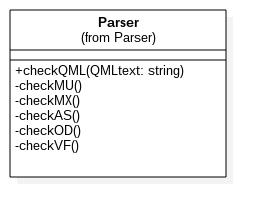
\includegraphics[scale=0.4]{../images/Model/Parser/Parser.png}
\end{center}
\end{figure}
\begin{itemize}
\item\textbf{Funzione del componente:} controlla che il testo fornito risulti corretto secondo la sintassi QML
\item\textbf{Relazioni d'uso con altre componenti:} 
Questo elemento è in relazione con:
\begin{itemize}
\item Model::Database::QuestionManager\\
\end{itemize}
\item\textbf{Metodi}:
le seguenti funzioni utilizzano le espressioni regolari per il controllo sintattico del codice QML.
Le espressioni regolari sono definite a livello globale come segue:\\
\begin{lstlisting}
var VF = /^[\s]*<question [\s]*type[\s]*=[\s]*"(VF)">[\s]*<text>[\s]*(.*)[\s]*<\/text>[\s]*<answer [\s]*isRight[\s]*=[\s]*"(yes|no)"[\s]*>(.*)<\/answer>[\s]*<\/question>[\s]*$/;

var MU = /^[\s]*<question [\s]*type[\s]*=[\s]*"(MU)">[\s]*<text>[\s]*(.*)[\s]*<\/text>(([\s]*<answer [\s]*isRight[\s]*=[\s]*"(yes|no)"[\s]*>(.*)<\/answer>[\s]*){2,})<\/question>[\s]*$/;

var MX = /^[\s]*<question [\s]*type[\s]*=[\s]*"(MX)">[\s]*<text>[\s]*(.*)[\s]*<\/text>(([\s]*<answer [\s]*isRight[\s]*=[\s]*"(yes|no)"[\s]*>(.*)<\/answer>[\s]*){2,})<\/question>[\s]*$/;

var AS = /^[\s]*<question [\s]*type[\s]*=[\s]*"(AS)">[\s]*<text>[\s]*(.*)[\s]*<\/text>[\s]*((<answer [\s]*set[\s]*=[\s]*"(A|B)" [\s]*pos[\s]*=[\s]*"(\d)"[\s]*>(.*)<\/answer>[\s]*){2,})<\/question>[\s]*$/;

var OD = /^[\s]*<question [\s]*type[\s]*=[\s]*"(OD)">[\s]*<text>[\s]*(.*)[\s]*<\/text>[\s]*((<answer [\s]*pos[\s]*=[\s]*"(\d)"[\s]*>(.*)<\/answer>[\s]*){2,})<\/question>[\s]*$/;

\end{lstlisting}
\newpage
	\begin{itemize}
		\item\code{+ checkQML()} : Metodo per controllare che un nuovo quesito rispetti la sintassi QML prima di essere aggiunto al database.\\
		\textbf{Parametri}: QMLText: string
		Il metodo prende in input il parametro QMLText di tipo string che rappresenta la stringa composta dall'utente in seguito al tentativo di creazione della domanda.
		
				\textbf{Precondizioni}: Viene richiesta una string che contiene la domanda\\
				\textbf{Postcondizioni}: Viene restituito un messaggio contenente il risultato dell'operazione di controllo sintattico\\
				
		\item\code{- checkMU()}: funzione che controlla se è presente una ed una sola risposta giusta\\
			
				
				\textbf{Precondizioni}: la funzione checkQML() ha preso in input il testo prodotto dall'utente ed è stata creata e definita la variabile m di tipo array che contiene i risultati della funzione exec() chiamata in checkQML()\\
				\textbf{Postcondizioni}: viene restituita una variabile di tipo bool riguardante l'esito positivo o negativo del controllo\\
			
		\item\code{- checkMX()}: funzione che controlla se sono presenti due o più risposte giuste\\
			\
				
				\textbf{Precondizioni}: la funzione checkQML() ha preso in input il testo prodotto dall'utente ed è stata creata e definita la variabile m di tipo array che contiene i risultati della funzione exec() chiamata in checkQML()\\
				\textbf{Postcondizioni}: viene restituita una variabile di tipo bool riguardante l'esito positivo o negativo del controllo\\
			
		\item\code{- checkAS()}: funzione che controlla la coerenza degli insiemi A e B definiti nella domanda prodotta dall'utente. Viene controllato che l'utente abbia dato agli insiemi i nomi corretti e sia stato definito un codice identificativo per ogni elemento di ciascun insieme\\
			
				\textbf{Precondizioni}: la funzione checkQML() ha preso in input il testo prodotto dall'utente ed è stata creata e definita la variabile m di tipo array che contiene i risultati della funzione exec() chiamata in checkQML()\\
				\textbf{Postcondizioni}: viene restituita una variabile di tipo bool riguardante l'esito positivo o negativo del controllo\\
			
		\item\code{- checkOD()}: funzione che controlla che ogni risposta abbia un codice identificativo univoco (in relazione alle altre risposte) in modo da poter effettuare l'ordinamento delle stesse\\
			\
				
				\textbf{Precondizioni}: la funzione checkQML() ha preso in input il testo prodotto dall'utente ed è stata creata e definita la variabile m di tipo array che contiene i risultati della funzione exec() chiamata in checkQML()\\
				\textbf{Postcondizioni}: viene restituita una variabile di tipo bool riguardante l'esito positivo o negativo del controllo\\
	\end{itemize}
\end{itemize}
\newpage

\subsubsection{La sintassi QML}
I seguenti metodi servono a controllare che la sintassi sia corretta secondo le regole QML.
Ogni domanda deve avere un tipo appartenente al seguente elenco:
\begin{itemize}
\item \textbf{VF}: domanda di tipo vero/falso
\item \textbf{MU}: domanda a risposta a scelta multipla con una sola risposta giusta
\item \textbf{MX}: domanda a risposta a scelta multipla con più risposte giuste
\item \textbf{AS}: domanda di associazioni tra elementi dell'insieme A ed elementi dell'insieme B
\item \textbf{OD}: domanda di ordinamento delle risposte date
\end{itemize}
Ogni domanda deve contenere i seguenti campi:
	\begin{itemize}
		\item Tipo domanda (VF, MU, MX, AS, OD)
		\item Testo della domanda
		\item Elenco risposte (di tipologia diversa in base al tipo di domanda)
		\item Percorso immagine allegata (opzionale)\\
	\end{itemize}

I suddetti campi vengono definiti nel modo seguente:\\
\begin{itemize}
\item <question type="VF|MU|MX|AS|OD" image="path/to/image"> ... </question> \\

Definisce l'inizio e la fine dell'oggetto domanda completo. L'attributo \textbf{type} definisce la tipologia di domanda che si vuole creare.
Nel caso si volesse allegare un'immagine alla domanda si deve aggiungere l'attributo \textbf{image} a cui va assegnato il percorso relativo dell'immagine da allegare.\\
\item <text> </text>\\
Per definire il campo relativo al testo della domanda
\item I campi per le risposte cambiano in base alla tipologia della domanda:\\

VF:\\
<answer isRight="yes|no"></answer>\\ Per il tipo vero/falso deve esserci un solo elemento risposta. 	L'attributo \textbf{isRight} definisce se la risposta è vera o falsa\\

MU:\\
 <answer isRight="yes|no"> risposta </answer>\\
Numero risposte > 1\\
Per ogni risposta va definito se è corretta o no. Il numero di risposte corrette deve essere = 1\\

		MX:\\
	<answer isRight="yes|no"> risposta </answer>\\
Numero risposte > 2\\
Per ogni risposta va definito se è corretta o no. Il numero di risposte corrette deve essere >= 1\\

		AS:\\
		<answer set="A" pos="1"> risp </answer>\\
Numero risposte > 1\\
Per ogni risposta va definito a che insieme appartiene tramite l'attributo \textbf{set}, e il numero identificativo di riferimento tramite l'attributo \textbf{pos}\\

		OD:\\
		<answer pos="1"> risp </answer>\\
Numero risposte > 1\\
Ad ogni risposta viene associata la sua posizione tramite la definizione dell'attributo \textbf{pos}
\end{itemize}
\newpage

\subsubsection{Esempi di domande secondo la sintassi corretta}
\begin{itemize}
\item Vero/Falso:\\
\begin{lstlisting}
<question type="VF">
	<text>
		testo della domanda
	</text>
	<answer isRight="yes"></answer>
</question>
\end{lstlisting}
\item Risposta multipla:\\
\begin{lstlisting}
<question type="MU">
    <text>
    	testo della domanda
    </text>
    <answer isRight="yes"> risp1 </answer>
    <answer isRight="no"> risp2 </answer>
    <answer isRight="no"> risp3 </answer>
</question>
\end{lstlisting}
\item Risposta multipla con più risposte corrette:
\begin{lstlisting}
<question type="MX"> 
	<text>
    	testo della domanda
    </text>
    <answer isRight="yes"> risp1 </answer>
    <answer isRight="yes"> risp2 </answer>
    <answer isRight="no"> risp3 </answer>
</question>
\end{lstlisting}
\item Associazione:
\begin{lstlisting}
<question type="AS"> 
	<text>
    	testo della domanda
    </text>
    <answer set="A" pos="1"> risp1 </answer>
    <answer set="A" pos="2"> risp2 </answer>
    <answer set="B" pos="1"> risp3 </answer>
    <answer set="B" pos="2"> risp4 </answer>
    <answer set="B" pos="3"> risp5 </answer>
</question>
\end{lstlisting}
\item Ordinamento:
\begin{lstlisting}
<question type="OD">
	<text>
    	testo della domanda
    </text>
	<answer pos="2"> risp2 </answer>    
    <answer pos="1"> risp1 </answer>
    <answer pos="3"> risp4 </answer>
    <answer pos="5"> risp6 </answer>
    <answer pos="4"> risp5 </answer>
</question>
\end{lstlisting}
\end{itemize}
\newpage

\subsection{Model::Statistics}
\subsubsection{Model::Statistics::Statistics}
\begin{figure}[h!]
\begin{center}
	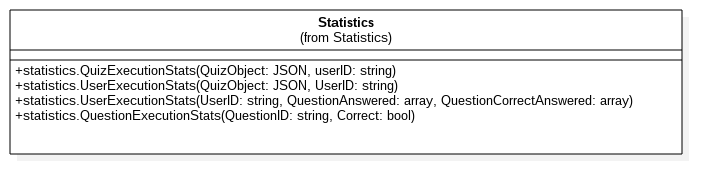
\includegraphics[scale=0.4]{../images/Model/Statistics/Statistics.png}
\end{center}
\end{figure}
\begin{itemize}
\item\textbf{Funzione del componente:} questa classe fornisce funzionalita' per il raccoglimento delle statistiche sulle prestazioni degli utenti del sistema
\item\textbf{Relazioni d'uso con altre componenti:}
Questo elemento è in relazione con:
\begin{itemize}
	\item Model::Publishers::QuizPublishers\\
	\item Model::Publishers::questionPublishers\\
\end{itemize}
\item\textbf{Metodi}:
\begin{itemize}
	\item\code{+ statistics.QuizExecutionStats()} : Metodo per aggiornare le statistiche di un quesito nel database\\
	\textbf{Parametri}:
	\begin{itemize}
		\item\code{QuizObject: JSON object}\\
		\item\code{UserID: string}\\
		\textbf{Precondizioni}: L'utente ha consegnato il questionario\\
		\textbf{Postcondizioni}: Le statistiche relative ad ogni domanda contenuta nel questionario sono state aggiornate\\
	\end{itemize}
	\item\code{+ statistics.UserExecutionStats()} : Metodo per aggiornare le statistiche sulla performance di un utente registrato\\
	\textbf{Parametri}:
	\begin{itemize}
		\item\code{UserID: string}\\
		\item\code{QuestionAnswered: array/string/int}\\
		\item\code{QuestionCorrectAnswered: array/string/int}\\
		\textbf{Precondizioni}: L'utente registrato ha consegnato un questionario\\
		\textbf{Postcondizioni}: Vengono aggiornate le statistiche totali di quell'utente\\
	\end{itemize}
	\item\code{+ statistics.QuestionExecutionStats()} : Metodo per aggiornare le statistiche di un quiz nel database\\
	\textbf{Parametri}:
	\begin{itemize}
		\item\code{QuestionID: string}\\
		\item\code{Correct: bool}\\
		\textbf{Precondizioni}: L'utente ha dato una risposta alla domana\\
		\textbf{Postcondizioni}:La risposta (corretta o meno) viene integrata nelle statistiche\\
	\end{itemize}
\end{itemize}
\end{itemize}
\newpage

\subsection{Model::Publishers}
\subsubsection{Model::Publishers::QuizPublisher}
\begin{figure}[h!]
\begin{center}
	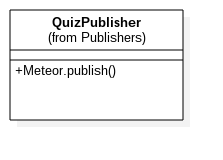
\includegraphics[scale=0.4]{../images/Model/Publishers/QuizPublisher.png}
\end{center}
\end{figure}
\begin{itemize}
\item\textbf{Funzione del componente:} questa classe fornisce funzionalita' per rendere pubblica la collezione dei quiz all'avvio del Sistema
\item\textbf{Relazioni d'uso con altre componenti:} Nessuna \\
\item\textbf{Metodi}:
	\begin{itemize}
		\item\code{+ Meteor.publish()} : Metodo per rendere accessibili la collezione dei quiz all'avvio del Sistema\\
		\textbf{Precondizioni}: Il Sistema non ha ancora reso pubblica la collezione dei quiz\\
		\textbf{Postcondizioni}: Il Sistema ha reso pubblica la collezione dei quiz\\
	\end{itemize}
\end{itemize}
\newpage

\subsubsection{Model::Publishers::QuestionPublisher}
\begin{figure}[h!]
\begin{center}
	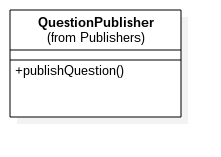
\includegraphics[scale=0.4]{../images/Model/Publishers/QuestionPublisher.png}
\end{center}
\end{figure}
\begin{itemize}
\item\textbf{Funzione del componente:} questa classe fornisce funzionalita' per rendere pubblica la collezione dei quesiti all'avvio del Sistema
\item\textbf{Relazioni d'uso con altre componenti:} Nessuna \\
\item\textbf{Metodi}:
	\begin{itemize}
		\item\code{+ publishQuestion()} : Metodo per rendere accessibili la collezione dei quesiti all'avvio del Sistema\\
		\textbf{Precondizioni}: Il Sistema non ha ancora reso pubblica la collezione dei quesiti\\
		\textbf{Postcondizioni}: Il Sistema ha reso pubblica la collezione dei quesiti\\
	\end{itemize}
\end{itemize}